\chapter{Présentation du travail réalisé} % Main chapter title

\label{Chapter3} % Change X to a consecutive number; for referencing this chapter elsewhere, use \ref{ChapterX}

\lhead{Chapitre 3. \emph{Présentation du travail réalisé}} % Change X to a consecutive number; this is for the header on each page - perhaps a shortened title
\section{Phase d'études}
Vu les raisons mentionnées dans la partie étude de l'existant, la fonctionnalité la plus importante dans ce projet était la gestion documentaire. Il existe de nombreuses solutions répondant à ce besoin, comme \textit{SharePoint de Microsoft}, \textit{FileNet d'IBM}, etc... La plupart de ces solutions sont payantes et souvent ne répondent pas à 100\% aux besoins des entreprises. Alors il existe des solutions alternatives open source: les gestionnaires de contenus appelés CMS (\textit{Content Management System}). L'open source gagne chaque année de nouveaux domaines d'applications. Les solutions proposées sont de plus en plus matures, et sont de vraies alternatives aux solutions historiques, propriétaires\cite{ged}. Pour faire le choix, j'ai procédé à une étude des solutions existantes.
\subsection{Étude des solutions}
De nos jours ils existent plusieurs gestionnaires de contenu. Les solutions proposées par ces derniers sont différentes les unes des autres.
Afin de bien choisir mon CMS, j'ai essayé de répondre aux questions publiées dans le livre\cite{Choisir}  \textit{200 questions pour choisir un CMS} de Smile\footnote{Smile est le premier intégrateur français et européen de solutions open source.}. Pendant leur passage à l'université Paris Ouest Nanterre La Défense pour un séminaire sur l'open source, ils nous ont beaucoup parler des CMS du marché ainsi que des livres blancs téléchargeables sur leur site web. 
Les questions\footnote{toutes les questions viennent du livre Smile\cite{choixPage}} auxquelles j'ai répondu et qui étaient intéressantes pour ce projet sont indiquées dans le tableau~\ref{questionsChoix}.\\

\begin{table}[h]
\centering
\begin{tabular}{|p{10cm}|m{2cm}|}
\hline questions & réponses \tabularnewline
\hline est-il possible de définir des types de contenus nouveaux, correspondant à un besoin spécifique & oui \tabularnewline
\hline est-il possible de modifier un type de contenu alors qu'il existe déjà de contenus de ce type & oui \tabularnewline
\hline est-il possible d'ajouter des méta-données & oui \tabularnewline
\hline est-il possible de définir l'arborescence du site, sans limitation de profondeur & oui \tabularnewline
\hline est-il possible de placer un même contenu dans plusieurs pages distinctes ? ceci sans le dupliquer & oui \tabularnewline
\hline est-il possible de gérer plusieurs sites au sein d'un unique back-office & oui \tabularnewline

\hline existe-t-il une médiathèque & oui \tabularnewline
\hline existe-t-il des fonctions de traitement d'images intégrées & oui \tabularnewline
\hline l'interface de contribution est-elle facile à prendre en main pour les non initiés & oui \tabularnewline
\hline est-il possible de définir des habilitations de validation distinctes selon les rubriques & oui \tabularnewline
\hline le valideur peut-il avoir un aperçu du contenu dans la page où il sera publié et avec le gabarit correspondant & oui \tabularnewline
\hline le CMS permet-il de produire des publications autres que Html\footnote{Hypertext Markup Langage est le format de données conçu pour représenter les pages web} ? par exemple pour les mobiles, pour les tablettes, etc. & oui \tabularnewline
\hline est-il possible de diffuser des contenus sous la forme de flux RSS\footnote{ces flux représente un moyen simple d'être tenu informé des nouveaux contenu d'un site web, sans avoir à le consulter\cite{ccm}} & oui \tabularnewline
\hline peut-on rendre certaines parties du site privatives pour des groupes ou utilisateurs & oui \tabularnewline
\hline les habilitations peuvent-elles être définies par groupes d'utilisateurs & oui \tabularnewline
\hline est-il possible de définir précisément les droits sur chacune des actions élémentaire de back-office & oui \tabularnewline
\hline le CMS possède-t-il une fonction de recherche intégrée & oui \tabularnewline
\hline peut-on gérer les utilisateurs depuis un annuaire LDAP\footnote{Protocole d'annuaire sur TCP/IP. Il permet de partager des bases d'informations sur le réseau interne ou externe\cite{ldap}} & oui \tabularnewline
\hline le produit est-il diffusé sous licence open source, ou bien sous une licence commerciale & open source \tabularnewline
\hline workflow pour notifier les utilisateurs & oui \tabularnewline
\hline
\end{tabular}

\caption{\label{questionsChoix}Questions pour choisir un CMS}
\end{table}
\clearpage


\subsection{Solution retenue}
Après avoir répondu à toutes les questions~\ref{questionsChoix}, j'ai regardé la comparaison effectuée par Smile dans le cadre de la présentation des différents CMS du marché\cite{comparaison}. La figure représente le résultat de cette comparaison.
\begin{figure}[h]
\centering
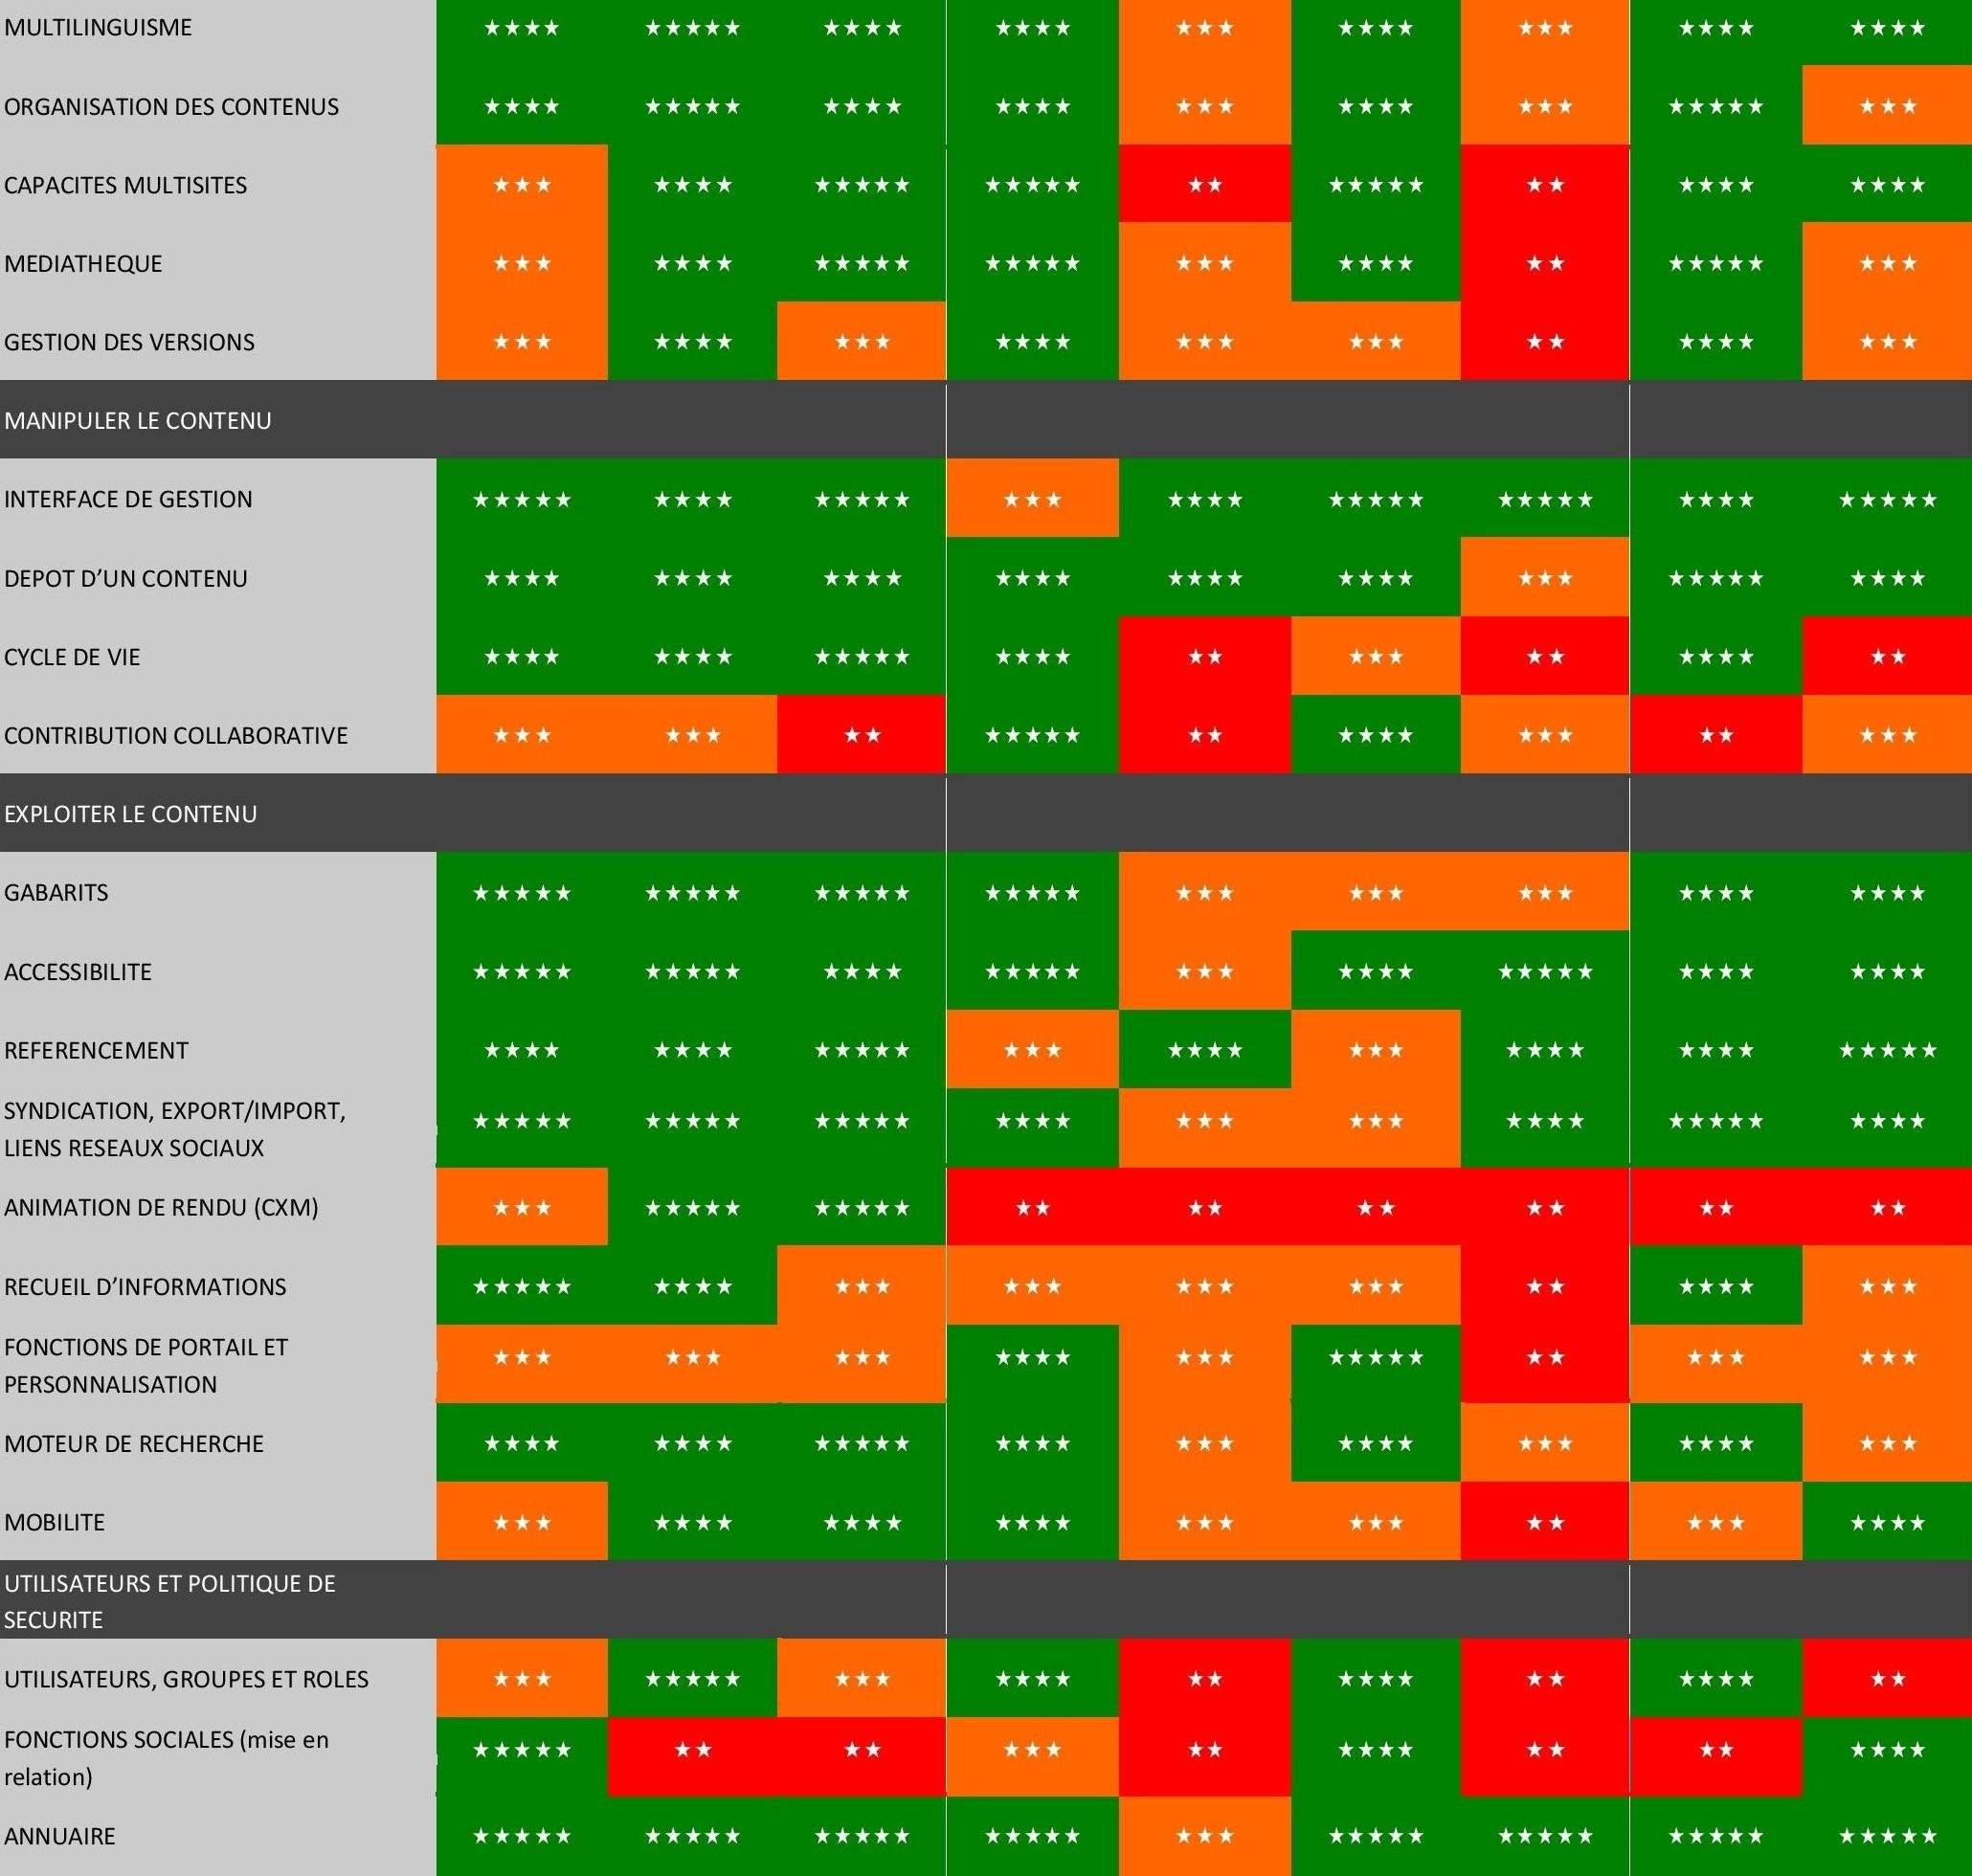
\includegraphics[width=14.5cm]{comparaison.jpg}
\caption{\label{comparaisonRef}Comparaison entre les CMS\cite{comparaison}}
\end{figure}
\clearpage
Après cette comparaison nous remarquons que les CMS qui se détachent des autres sont:
\begin{itemize}
\item Typo3: qui est un très bon gestionnaire de contenu mais il n'a pas été retenu parce qu'il est moins performant sur les \og Portails Intranet\fg{}\cite{typo3} et aussi il ne nous permettait pas d'organiser notre portail sous forme d'espace.
\item Jahia: a un très beau score dans le tableau de comparaison, mais ce CMS n'a pas été retenu parce qu'il ne permettait pas d'organiser notre portail sous forme d'espace.
\item Ez publish: obtient lui également un beau score dans la comparaison, en revanche il n'est pas assez documenter.
\item Drupal: même s'il reste un peu en retrait sur la mise en place d'une architecture multi-sites, drupal a été la solution que nous avons choisi car il est très bien documenté, il y a une forte communauté derrière pour assurer le bon fonctionnement de ce CMS et aussi propose plusieurs modules dont \og open atrium\fg{} qui répondent parfaitement à nos besoins. \\Sans me le dire lors de ma phase d'étude pour le choix du CMS, mon tuteur en entreprise avait également fait des recherches par rapport au type de CMS que je pouvais utiliser et c'est Drupal qu'il avait choisi.
\end{itemize}
\section{Développement}
La phase de développement fut l'une des phases les plus importantes dans ce projet, car elle sert à mettre en place l'outil demandé grâce aux différentes solutions qui ont été retenues.\\
Durant le développement, plusieurs réunions avec les futurs utilisateurs ont été organisée car on travaillait en méthode agile, donc à la fin de chaque une itération, les utilisateurs devaient tester la ou les fonctionnalités développées puis les valider si elle(s) répond(ent) à leur besoins.\\
Dans cette partie nous allons parler des fonctionnalités qui ont pu être réalisées et également celles qui n'ont pas pu l'être.
\subsection*{Tâches réalisées}
Avant de commencer à réaliser le développement, nous avons effectué quelques réunions avec les super utilisateurs\footnote{les super utilisateurs sont les personnes représentants les différents profils (BERE, MOAD) }. 
Le but de ces réunions était de pouvoir comprendre ce que les clients voulaient et de s'assurer qu'on a bien compris ce qu'ils voulaient. Au bout de 3 réunions, nous avons dressé une nouvelle liste de fonctionnalités avec des priorités différentes. Ces fonctionnalités n'étaient pas définitives, car elles pouvaient être modifiées par rapport à la faisabilité ou au besoin.
La nouvelle liste de fonctions à réaliser était: 
\begin{itemize}
\item l'authentification via l'annuaire \textbf{\textit{GARDIAN SESAME}}: tout accès au portail devait passer par l'annuaire gardian sesame afin de sécuriser le site. Cette tâche avait une priorité élevée car tous leurs outils utilisaient ce système d'authentification, donc il n'était pas question de réaliser un autre outil avec un autre système d'authentification.\\
Pour accomplir cette tâche j'avais chercher des modules drupal permettant de gérer les connexions LDAP, mais les modules trouvés ne prenait pas en compte le type d'authentification que je devais réalisé. Alors pour résoudre ce problème j'ai dû aller dans le cœur de drupal pour modifier le système de connexion.
\begin{lstlisting}
	<?php
	// inclusion des classes necessaires
	// pour l'authententification LDAP 
	include("ldap/LdapAuth.php");
	$options= array(
	// liste des serveurs LDAP sur lesquels on doit tenter 
	//la connexion pour authentification. 
	//L'ordre est important.
	'servers' => array("lien-annuaire-1","lien-annuaire-2"),
	'use_ldaps'=> true,
	'bind_dn'=> "uid=identApp,ou=ou-1,dc=mydc",
	'bind_pwd'=> 'XXXXXXX',
	// base de recherche dans l'annuaire 
	//pour la recherche d'utilisateur
	'searchBase'=> "ou=ou-2,dc=mydc",
	// fermeture automatique de la 
	//connection LDAP a la fin de 
	//l'authentification (utile si 
	//plusieurs authentification dans le script)
	'closeConnection'	=> true,
	// delai maximum de recherche LDAP (pour la recherche 
	//de l'utilisateur pour recuperation du DN)
	'timelimit'=> 1
	);
	$ldapAuth=new LdapAuth($options);
	
	try {
		$nni = $form_state['values']['name'];
		$pass = $password;
		$date = date('Y-m-d H:i:s');
		$ldapbind=$ldapAuth->authenticateUser($nni, $pass);
		
	} catch (LdapException $e) {
	 
		$resultat=$e->getMessage();
	}
\end{lstlisting}
\item les espaces: dans le portail, on avait plusieurs profil (moad, bere, public, hypervision, commun) et rôle; donc chaque profil avait son propre espace de travail.
\item la gestion des droits: on avait différents rôles et groupes de travail dans chaque espace, donc on devait pouvoir gérer les droits des utilisateurs en fonctions des groupes qu'ils appartiennent ou des rôles qu'ils possèdent selon l'espace dans lequel ils se trouvent. Cette fonctionnalité avait également une priorité élevée  
\item trombinoscope: avec une priorité moyenne, cette fonctionnalité permet aux utilisateurs de retrouver facilement les contacts des autres utilisateurs. Comme drupal fonctionne avec des modules, nous avons mis en place un module permettant de récupérer les informations (nom, prénom, mail, photo, téléphone) des utilisateurs et de les afficher selon la demande de l'utilisateur.
\item gestion documentaire: elle était la partie la plus importante du projet, les utilisateurs devaient pouvoir partager leurs documents dans leur espace tout en gérant également les droits de lecture et d'écriture sur ces documents avec des systèmes de notification selon qu'on soit abonné ou pas. Alors pour cette fonctionnalité, on avait opté pour une première solution qui consiste à utiliser filedepot\footnote{filedepot est un module de gestionnaire de fichier sous drupal}. Après avoir mise en place cette solution, les clients l'ont jugé un peu compliquée, alors nous avons développé une autre solution plus simple que la première tout en gardant la première solution au cas où on voudra revenir la dessus car cette dernière présente de nombreuses fonctionnalités intéressantes.
\item gestion de types de contenus: l'administrateur devait pouvoir créer différents types de contenus comme par exemple un article avec des photos, des liens vers d'autres documents etc... De natif, drupal gère la gestion des types de contenus, donc la mise en place de cette solution n'a pas été compliquée
\item forum: le forum permet aux utilisateurs de pouvoir échanger par rapport à un sujet. Cette fonctionnalité avait une priorité faible. 
\item foires aux questions: comme pour le forum, cette fonctionnalité avait également une priorité faible. Elle a été réalisée grâce à un module FAQ de drupal.
\item gestion des réservations: avant, les utilisateurs utilisaient un fichier excel pour réservation des voitures, des salles de conférences, des bureaux etc. Alors on a intégré dans notre outil un système de réservation plus simple et plus fiable. Cette fonctionnalité avait une priorité élevée.
\item tableau de bord: ce tableau permettait à l'hyperviseur de voir les statistiques sous forme de graphes, camembert etc. Elle avait une priorité élevée.
\item carte: avec une priorité élevée, on devait afficher sur la carte les différents postes sources avec leurs informations (liens vers les études correspondantes aux postes sources, le nombre de clients etc...)
\item formulaire de demande: ce formulaire de demande servait en quelque sorte comme un outil de suivi de projet ou de tâches. Les utilisateurs peuvent s'adresser entre eux, des demandes de tâches et en même temps suivre l'état d'avancement des tâches demandées. cette fonctionnalité avait une faible priorité.
\end{itemize}
\subsection*{Tâches non réalisées}\label{nonrealise}
Parmi les fonctionnalités citées ci-dessus, la plupart a été réalisée sauf deux qui sont: 
\begin{itemize}
\item tableau de bord: le tableau de bord n'a pas pu être réalisée car c'est mon tuteur en entreprise qui devait me fournir la liste des données ainsi que les types de calculs qu'on devait faire pour les statistiques. Malheureusement vers la fin du mois de juillet, il est tombé malade et il n'est retourné qu'au mois de septembre. En son absence, on a chargé une autre personne de s'occuper du suivi de projet mais ce dernière était également en congé et elle n'est retournée que vers mi-août. Alors cette personne n'étant pas au courant de la réalisation du tableau de bord, elle ne pouvait pas m'aider car elle n'avait pas connaissance des données qu'on devait récupérer pour faire les statistiques.\\
On a fait quand même un exemple de tableau de bord avec des données statiques pour montrer que c'était faisable.
\item carte: pour les mêmes raisons que le tableau de bord, l'absence de mon tuteur à mis en suspension la réalisation de cette fonctionnalité car c'est lui qui devait me fournir le reste des éléments pour faire la carte. On avait déjà commencé à réaliser cette fonctionnalité, une grande partie ayant été faite, ils (les utilisateurs) pourront eux même continuer avec le reste car il n'y a plus de code à faire mais juste la saisie des données.
\end{itemize}
